\documentclass[11pt,a4paper]{article}
\usepackage[T1]{fontenc}
\usepackage{lmodern}
\usepackage[margin=2.5cm]{geometry}
\usepackage{amsmath,amssymb,amsthm,mathtools}
\usepackage{cryptocode}
\usepackage{booktabs,array,tabularx}
\usepackage{graphicx}
\usepackage{tikz}
\usetikzlibrary{arrows.meta,positioning,shapes.geometric,calc,fit}
\usepackage{microtype}
\usepackage{xcolor}
\usepackage[colorlinks=true,linkcolor=blue!50!black,citecolor=blue!50!black,urlcolor=blue!50!black]{hyperref}
\usepackage[capitalise,noabbrev]{cleveref}
\usepackage{enumitem}
\setlist{itemsep=2pt,topsep=4pt}

\newcommand{\demourl}{SAKSI_DEMO_URL}
\newcommand{\repourl}{SAKSI_REPO_URL}

\theoremstyle{plain}
\newtheorem{theorem}{Theorem}
\newtheorem{lemma}[theorem]{Lemma}
\newtheorem{proposition}[theorem]{Proposition}
\newtheorem{corollary}[theorem]{Corollary}
\theoremstyle{definition}
\newtheorem{definition}{Definition}
\newtheorem{remark}{Remark}

\newcommand{\F}{\mathbb{F}_p}
\newcommand{\ctx}{\mathsf{ctx}}
\newcommand{\Vote}{\mathsf{votes}}
\newcommand{\bad}{\bot}
\providecommand{\adv}{\mathcal{A}}
\providecommand{\sample}{\xleftarrow{\$}}
\DeclareMathOperator{\Syn}{Syn}

% AUTO-GENERATED by gen_results.py from attacks/results/*.json -- do not edit
\newcommand{\EonePrimes}{$(p,t)=(31,3)$, $(p,t)=(101,2)$, $(p,t)=(13,4)$}
\newcommand{\EoneAllIdentical}{Yes}
\newcommand{\EtwoN}{100{,}000}
\newcommand{\EtwoBins}{256}
\newcommand{\EtwoP}{0.297, 0.941, 0.885}
\newcommand{\EtwoMIbiased}{0.0056}
\newcommand{\EtwoMIuniform}{0.0}
\newcommand{\EthreeSaksiCand}{31}
\newcommand{\EthreeSaksiSpace}{31}
\newcommand{\EthreeSaksiBits}{0.00}
\newcommand{\EthreeMigCand}{14}
\newcommand{\EthreeMigSpace}{1{,}993}
\newcommand{\EthreeMigBits}{7.15}
\newcommand{\EfourTrials}{200{,}000}
\newcommand{\EfourMaxDev}{0.0010}
\newcommand{\EfiveBitflip}{81.9\%}
\newcommand{\EsixTrials}{150}
\newcommand{\EsixCorrect}{100.0\%}
\newcommand{\EsixWrong}{0.0\%}
\newcommand{\EsixNamed}{100.0\%}
\newcommand{\EsevenN}{2{,}000}
\newcommand{\EsevenCrash}{0}
\newcommand{\EsevenWrong}{0}
\newcommand{\EeightT}{380.2}
\newcommand{\EeightN}{200{,}000}
\newcommand{\BenchMul}{9.0}
\newcommand{\BenchInv}{2.43}
\newcommand{\BenchDeal}{40.8}
\newcommand{\BenchRec}{45.2}
\newcommand{\BenchKeyless}{62.6}
\newcommand{\TimingMaxCore}{1.11}
\newcommand{\TimingMinCtrl}{192}
\newcommand{\TimingSamples}{1{,}000{,}000}
\newcommand{\RushTrials}{500}
\newcommand{\RushOneRound}{100.0\%}
\newcommand{\RushSyndrome}{100.0\%}
\newcommand{\RushTwoRound}{0.0\%}
\newcommand{\BoundWrong}{100.0\%}
\newcommand{\BoundClosed}{0.0\%}
\newcommand{\BoundTrials}{100}


\title{\textbf{SAKSI}: Witness-Validated Secret Sharing with\\Unconditional Cheater Identification over $\mathrm{GF}(2^{127}-1)$}
\author{Shermaine Yap Shi Min\\[2pt]
\small Asia Pacific University of Technology and Innovation (APU), Kuala Lumpur, Malaysia}
\date{November 2026}

\begin{document}
\maketitle

\begin{abstract}
A master key that exists in one place is one compromise away from total loss, and a key that is
split with plain Shamir sharing can be silently corrupted: a single dishonest share-holder can
make everyone else reconstruct garbage while learning the real key itself (the Tompa--Woll
attack). We present \textbf{SAKSI} (Malay: \emph{witness}), a $(t,n)$ secret-sharing scheme for
master keys over the Mersenne prime field $\F$, $p=2^{127}-1$, that \emph{validates} every share
before it is used. Each share carries one-time affine \emph{witness tags}, one per other custodian,
bound to a public context (session, epoch, index) and checked in a two-round reveal; a
generalised Reed--Solomon syndrome independently cross-checks the accepted shares and Gao decoding
localises any residual inconsistency, including a dishonest dealer. Secrecy is perfect, a forged
share passes a single witness with probability exactly $1/p=2^{-127}$, and with at most
$\lfloor (n-1)/2\rfloor$ cheaters the correct key is returned and every modified share is named,
except with probability at most $2^n/p$. No block cipher, hash function or computational
assumption is used anywhere, so the guarantees hold against computationally unbounded (including
quantum) adversaries. The core is written in branch-free Rust; a dudect leakage study over up to
\TimingSamples{} measurements finds no timing dependence on secrets ($|t|\le\TimingMaxCore$),
while deliberately leaky controls are flagged ($|t|\ge\TimingMinCtrl$). An attack harness of eight
experiments, including Z3-assisted collusion and active tampering on the real parameters, is
published with the code, and the scheme is deployed in a browser agent that can use an API
credential only after validated reconstruction.
\end{abstract}

\section{Introduction}\label{sec:intro}

Threshold secret sharing~\cite{shamir79,blakley79} removes the single point of failure of a master
key: the key is encoded into $n$ shares such that any $t$ of them recover it and any $t-1$ reveal
nothing. Plain Shamir sharing, however, gives no way to tell a correct share from a wrong one.
Tompa and Woll~\cite{tompawoll88} showed that the last participant to submit can choose a share so
that the others reconstruct a wrong value while the cheater, knowing what it submitted, recovers
the true secret. Data corruption, a buggy custodian or a malicious insider all look the same to
Lagrange interpolation: it always returns \emph{some} key.

This matters for key custody in software agents. An AI agent that needs a credential should never
hold it permanently, and the provider of the language model it talks to should never see it.
Splitting the credential across custodians solves the first problem only if reconstruction is
\emph{validated}: a corrupted share must be detected and attributed, and the system must fail
closed rather than use a wrong key.

\paragraph{What is from the literature.}
Polynomial sharing over a field is Shamir's~\cite{shamir79}. Information-theoretic ``check
vectors'' that let one player authenticate another's share are due to Rabin and
Ben-Or~\cite{rabinbenor89}; robust sharing with short tags and the role of rushing adversaries are
analysed by Cevallos et al.~\cite{cfor12}. The relation between Shamir shares and Reed--Solomon
codewords and Gao's decoder are classical~\cite{gao02}. Proactive refresh by adding a sharing of
zero is due to Herzberg et al.~\cite{herzberg95}. Computational verifiable secret sharing
(Feldman~\cite{feldman87}, Pedersen~\cite{pedersen91}) and CRT-based sharing
(Mignotte~\cite{mignotte83}, Asmuth--Bloom~\cite{asmuthbloom83}) are the main alternatives.

\paragraph{Contributions.}
\begin{enumerate}
  \item \textbf{A concrete, fully specified construction} combining (i) Vandermonde/Shamir encoding over
  the Mersenne field $2^{127}-1$ in 120-bit limbs, (ii) \emph{context-bound inner-product witness
  tags} $\tau_{j,i}=\beta+\alpha_0\ctx_i+\sum_\ell\alpha_\ell y_{i,\ell}$ that authenticate the whole
  multi-limb share \emph{and} its session, epoch and index with a single field element,
  (iii) a two-round reveal with a $\lfloor (n-1)/2\rfloor$ vouching rule, and (iv) a parity-check
  (syndrome) cross-check with Gao decoding, plus a keyless Reed--Solomon fallback.
  \item \textbf{Proofs} of perfect secrecy including the tags, an exact forgery bound, robustness with
  cheater identification, and the necessity of the two-round order (\cref{sec:security}).
  \item \textbf{A constant-time Rust implementation} of the Mersenne arithmetic with a published
  dudect-style leakage study and positive controls (\cref{sec:sidechannel}).
  \item \textbf{An open attack harness} (eight experiments) that attacks SAKSI next to unvalidated
  controls (\cref{sec:experiments}).
  \item \textbf{Deployment} in a browser agent that custodies an API credential (\cref{sec:applied}).
\end{enumerate}
The individual ingredients are textbook; the contribution is a careful, minimal combination
specified down to the wire format, with proofs that match the code line by line and measurements
that test the claims.

\section{Preliminaries and threat model}\label{sec:prelim}

\paragraph{Notation.} $p=2^{127}-1$ is prime and $\F$ is the field of integers modulo $p$. Custodians
are indexed $i\in[n]=\{1,\dots,n\}$ and custodian $i$ is associated with the public evaluation
point $x_i=i$. A secret $S$ of $\lambda$ bytes is split into $L=\lceil\lambda/15\rceil$ limbs
$s_1,\dots,s_L\in[0,2^{120})\subset\F$ (big-endian, zero padded). The public header is
$H=(n,t,L,\lambda,\mathsf{sid},e)$ with a uniformly random session identifier $\mathsf{sid}\in\{0,\dots,2^{53}-1\}$ (53 bits so that it round-trips exactly through JSON and JavaScript numbers in the browser demo) and epoch
$e$. The public context of share $i$ is the field element
\[
  \ctx_i \;=\; \mathsf{sid} \;+\; 2^{64}e \;+\; 2^{96} i \qquad (\mathsf{sid}<2^{53}\le 2^{64},\ e<2^{32},\ i<2^{16}),
\]
an injective encoding of $(\mathsf{sid},e,i)$ into $[0,2^{112})\subset\F$.

\paragraph{Parties and channels.} A dealer runs $\mathsf{Deal}$ once per epoch and is trusted for that
epoch (as in Shamir sharing). Reconstruction is performed by a combiner that receives messages from
the custodians over \emph{authenticated} channels (the combiner knows which custodian sent which
message) and enforces two ordered rounds: no key from round~2 is released before every round-1
message has been fixed. If the channel is not authenticated and two shares arrive under the same
index (a cheater racing an honest custodian), the combiner keeps the candidate with the most witness
confirmations; a forgery under a stolen index therefore cannot displace the honest share (tested in
both implementations).

\paragraph{Adversary.} A static adversary $\adv$ corrupts a set $C\subseteq[n]$ of $c=|C|$
custodians before dealing, sees their entire state, and controls everything they send. It may be
\emph{rushing} within a round (it sees honest messages of the current round before choosing its
own), but cannot change a round-1 message after round 2 starts. It is computationally unbounded.
Robustness requires $c\le T\coloneqq\lfloor (n-1)/2\rfloor$ and $t\le n-c$; privacy requires
$c\le t-1$.

\begin{definition}[Properties]\label{def:props}
\textbf{Privacy:} the joint view of any $c\le t-1$ custodians before reconstruction is independent of
$S$. \textbf{Correctness:} if all custodians are honest, reconstruction from any $t$ of them outputs
$S$. \textbf{Robustness:} with at most $T$ corrupted custodians, reconstruction outputs $S$ or
fails closed ($\bad$), and outputs $S$ whenever at least $t$ honest custodians respond.
\textbf{Identification:} every corrupted custodian whose round-1 share differs from the dealt
share is reported.
\end{definition}

\section{The scheme}\label{sec:scheme}

\subsection{Algorithms}

\begin{figure}[ht]
\centering
\procedure[linenumbering]{$\mathsf{Deal}(S, n, t)$}{%
\textbf{assert }2\le t\le n,\ n\ge 3,\ S\ne\varepsilon \\
(s_1,\dots,s_L) \gets \mathsf{Limbs}_{15}(S);\quad \mathsf{sid}\sample\{0,\dots,2^{53}-1\};\quad e\gets 0\\
\pcfor \ell=1..L \pcdo \\
\pcind a_{\ell,0}\gets s_\ell;\quad a_{\ell,1},\dots,a_{\ell,t-1}\sample\F \\
\pcfor i=1..n \pcdo \\
\pcind y_{i,\ell}\gets \textstyle\sum_{k=0}^{t-1} a_{\ell,k}\, i^k \quad\text{(i.e.\ } \mathbf y_\ell = V\mathbf a_\ell\text{)}\\
\pcreturn \mathsf{Witness}(H, \{\mathbf y_i\}_{i\in[n]})
}

\medskip
\procedure[linenumbering]{$\mathsf{Witness}(H, \{\mathbf y_i\})$}{%
\pcfor \text{ordered } (j,i),\ j\ne i \pcdo \\
\pcind \kappa_{j,i}=(\alpha_0,\dots,\alpha_L,\beta)\sample\F^{L+2}\\
\pcind \tau_{j,i}\gets \beta+\alpha_0\ctx_i+\textstyle\sum_{\ell=1}^{L}\alpha_\ell y_{i,\ell}\\
\text{custodian } i \text{ gets } \big(\mathbf y_i, \{\tau_{j,i}\}_{j\ne i}\big)\\
\text{custodian } j \text{ gets } \{\kappa_{j,i}\}_{i\ne j}\\
\pcreturn \text{all custodian states}
}
\caption{Dealing. $V$ is the $n\times t$ Vandermonde matrix $V_{ik}=i^k$. All randomness comes
from the operating-system CSPRNG; field elements are sampled by rejection from 127 random bits
(rejecting only the value $p$).}
\label{fig:deal}
\end{figure}

\begin{figure}[ht]
\centering
\procedure[linenumbering]{$\mathsf{Reconstruct}(H)$}{%
\text{\textbf{Round 1:} each responding } i \text{ sends } (i,\mathbf y_i,\{\tau_{j,i}\}_j)
\text{; drop malformed shares and } y\notin[0,p)\\
\text{if several shares claim index } i\text{, keep the one with most votes (after round 2)}\\
\text{\textbf{Round 2:} each responding } j \text{ sends } \{\kappa_{j,i}\}_i\\
\pcfor \text{each received share } i \pcdo \\
\pcind \Vote_i \gets \#\{ j\ne i : \tau_{j,i} \overset{\mathrm{ct}}{=} \beta_{j,i}+\alpha_{j,i,0}\ctx_i+\textstyle\sum_\ell\alpha_{j,i,\ell}\, y_{i,\ell}\}\\
A\gets\{i : \Vote_i\ge T\};\quad \text{report } [n]\cap\{\text{received}\}\setminus A \text{ as rejected}\\
\pcif |A|<t \pcthen \pcreturn \bad \\
\pcif \Syn_A(\mathbf y_\ell)=\mathbf 0 \text{ for all } \ell \pcthen
  s_\ell\gets\textstyle\sum_{i\in A_t}\lambda_i y_{i,\ell} \quad(A_t=\text{first } t \text{ of } A)\\
\pcelse (f_\ell, E_\ell)\gets\mathsf{Gao}(A, \mathbf y_\ell, t) \text{ for all } \ell;\ \pcif \text{any fails} \pcthen \pcreturn\bad\\
\pcind s_\ell \gets f_\ell(0);\ \text{report } \cup_\ell E_\ell \text{ as located};\ \pcif |A\setminus\cup E_\ell|<t \pcthen\pcreturn\bad\\
\pcif \text{any } s_\ell\ge 2^{120} \text{ or padding}\neq 0 \pcthen \pcreturn \bad \quad\text{(encoding sanity check)}\\
\pcreturn S=\mathsf{Bytes}_\lambda(s_1,\dots,s_L)
}
\caption{Two-round reconstruction. $T=\lfloor(n-1)/2\rfloor$; $\lambda_i=\prod_{j\ne i}x_j/(x_j-x_i)$
are the Lagrange coefficients at $0$; $\Syn$ is defined in \cref{eq:syn}. $\mathsf{Reconstruct}_{\text{keyless}}$
skips the votes and runs $\mathsf{Gao}$ on all well-formed shares.}
\label{fig:rec}
\end{figure}

\paragraph{Syndrome.} For a set $A=\{x_1,\dots,x_m\}$ of distinct points and values
$\mathbf y\in\F^m$ define
\begin{equation}\label{eq:syn}
  \Syn_A(\mathbf y)_k \;=\; \sum_{i=1}^m v_i\, x_i^k\, y_i\quad (k=0,\dots,m-t-1),
  \qquad v_i=\prod_{j\ne i}(x_i-x_j)^{-1}.
\end{equation}
This is the parity-check matrix $H_A=\big(v_i x_i^k\big)$ of the generalised Reed--Solomon code
$\mathcal C_A=\{(f(x_1),\dots,f(x_m)):\deg f<t\}$; see \cref{lem:syn}.

\paragraph{Refresh.} $\mathsf{Refresh}$ samples $z_\ell(X)=\sum_{k=1}^{t-1}b_{\ell,k}X^k$ (so
$z_\ell(0)=0$), sets $y'_{i,\ell}=y_{i,\ell}+z_\ell(i)$, increments the epoch $e\gets e+1$ and calls
$\mathsf{Witness}$ again with fresh one-time keys.

\paragraph{Encoding sanity check.} An honest reconstruction always produces limbs below $2^{120}$
with zero padding. If a wrong limb appears (possible only beyond the robustness bound), it lies in
$[0,2^{120})$ with probability $2^{120}/p\approx2^{-7}$, so the check rejects it with probability
about $1-2^{-7}$ per limb. This is a heuristic extra layer; none of the proofs rely on it.

\begin{figure}[ht]
\centering
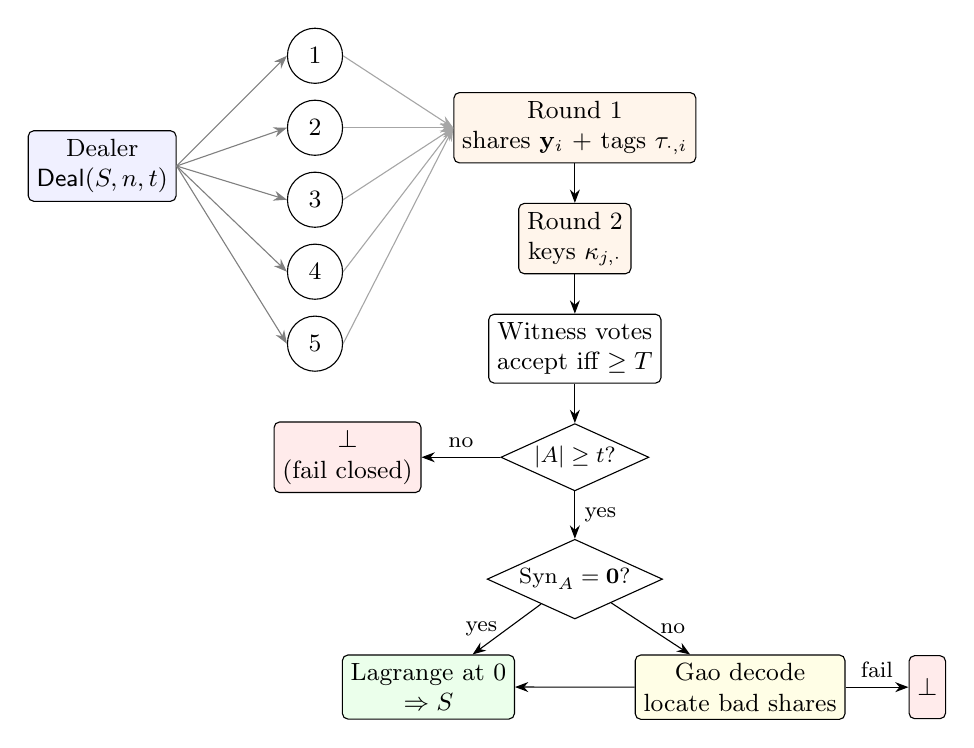
\begin{tikzpicture}[
  node distance=6mm and 6mm, >=Stealth,
  box/.style={draw, rounded corners=2pt, align=center, font=\small, minimum height=8mm, inner sep=3pt},
  cust/.style={draw, circle, font=\small, minimum size=7mm, inner sep=0pt},
  dec/.style={draw, diamond, aspect=2.2, align=center, font=\footnotesize, inner sep=1pt}]
\node[box, fill=blue!6] (dealer) {Dealer\\$\mathsf{Deal}(S,n,t)$};
\node[cust, right=14mm of dealer, yshift=14mm] (c1) {$1$};
\node[cust, below=2mm of c1] (c2) {$2$};
\node[cust, below=2mm of c2] (c3) {$3$};
\node[cust, below=2mm of c3] (c4) {$4$};
\node[cust, below=2mm of c4] (c5) {$5$};
\foreach \c in {c1,c2,c3,c4,c5} \draw[->, gray] (dealer.east) -- (\c.west);
\node[box, right=14mm of c2, fill=orange!8] (r1) {Round 1\\shares $\mathbf y_i$ + tags $\tau_{\cdot,i}$};
\node[box, below=5mm of r1, fill=orange!8] (r2) {Round 2\\keys $\kappa_{j,\cdot}$};
\foreach \c in {c1,c2,c3,c4,c5} \draw[->, gray!70] (\c.east) -- (r1.west);
\draw[->] (r1) -- (r2);
\node[box, below=5mm of r2] (votes) {Witness votes\\accept iff $\ge T$};
\draw[->] (r2) -- (votes);
\node[dec, below=5mm of votes] (enough) {$|A|\ge t$?};
\draw[->] (votes) -- (enough);
\node[box, left=10mm of enough, fill=red!8] (fail1) {$\bot$\\(fail closed)};
\draw[->] (enough) -- node[above, font=\footnotesize]{no} (fail1);
\node[dec, below=6mm of enough] (syn) {$\Syn_A=\mathbf 0$?};
\draw[->] (enough) -- node[right, font=\footnotesize]{yes} (syn);
\node[box, below left=7mm and 2mm of syn, fill=green!8] (lag) {Lagrange at $0$\\$\Rightarrow S$};
\node[box, below right=7mm and 2mm of syn, fill=yellow!10] (gao) {Gao decode\\locate bad shares};
\draw[->] (syn) -- node[left, font=\footnotesize]{yes} (lag);
\draw[->] (syn) -- node[right, font=\footnotesize]{no} (gao);
\node[box, right=8mm of gao, fill=red!8] (fail2) {$\bot$};
\draw[->] (gao) -- node[above, font=\footnotesize]{fail} (fail2);
\draw[->] (gao.west) -- (lag.east);
\end{tikzpicture}
\caption{Protocol flow of SAKSI for $n=5$. Rejected and located custodians are reported by index.}
\label{fig:flow}
\end{figure}

\subsection{Worked example (toy parameters)}\label{sec:toy}
Take $p=97$, $n=5$, $t=3$, a single limb $s=42$ and coefficients $a_1=11$, $a_2=7$, i.e.\
$f(X)=42+11X+7X^2$. The shares are
\[
  (y_1,\dots,y_5)=(60,\,92,\,41,\,4,\,78).
\]
\emph{Reconstruction.} For $A_t=\{1,2,3\}$ the Lagrange coefficients at $0$ are
$(\lambda_1,\lambda_2,\lambda_3)=(3,94,1)$ and $3\cdot60+94\cdot92+1\cdot41\equiv42\pmod{97}$.
\emph{Syndrome.} For all five points $v=(93,16,73,16,93)$ and $\Syn(\mathbf y)=(0,0)$. If custodian 4
changes $y_4$ to $9$, the syndrome becomes $(80,29)\neq\mathbf 0$, and Gao decoding (which corrects
$\lfloor(5-3)/2\rfloor=1$ error) returns $f$ and locates index~4.
\emph{Witness.} With toy key $(\alpha_0,\alpha_1,\beta)=(23,58,64)$ and toy context $\ctx_2=2$, the tag of
share~2 is $\tau=64+23\cdot2+58\cdot92\equiv14$. The shifted share $y_2+1=93$ evaluates to $72\ne14$
(the difference is exactly $\alpha_1=58$, which the cheater does not know).
\emph{Tompa--Woll on plain Shamir.} If custodian 3 adds $1$ to its share, plain interpolation over
$\{1,2,3\}$ returns $43$ instead of $42$; the cheater knows $\lambda_3=1$ and therefore the true key.

\subsection{Parameters and cost}
For a 32-byte key ($L=3$) and $n=5$, each custodian stores its share ($L$ elements), $n-1$ tags and
$n-1$ keys of $L+2$ elements: $3+4+4\cdot5=27$ field elements, i.e.\ 432 bytes. Key material is
$\Theta(n^2L)$ in total, which is the price of unconditional validation (\cref{sec:limits}).

\section{Security analysis}\label{sec:security}

\begin{theorem}[Perfect secrecy, including tags]\label{thm:privacy}
For every coalition $C$ with $|C|\le t-1$ and every two secrets $S,S'$ of equal length, the joint
view of $C$ after $\mathsf{Deal}$ (shares, tags, keys and header) has the same distribution
under $S$ and $S'$.
\end{theorem}
\begin{proof}
Limbs are shared with independent polynomials, so it suffices to treat one limb. Fix $s$ and the
values $(y_i)_{i\in C}$. The non-constant coefficients $(a_1,\dots,a_{t-1})$ must satisfy
$\sum_{k=1}^{t-1}a_k x_i^k = y_i - s$ for $i\in C$. The coefficient matrix
$(x_i^k)_{i\in C,\,1\le k\le t-1}=\operatorname{diag}(x_i)\cdot(x_i^{k-1})$ has full row rank $|C|$
because the $x_i$ are distinct and non-zero (a Vandermonde matrix times an invertible diagonal).
Hence exactly $p^{\,t-1-|C|}$ coefficient vectors are consistent with the view, independently of
$s$: the shares of $C$ are uniform on $\F^{|C|}$ and independent of $s$.
The keys held by $C$ are sampled independently of everything else. A tag $\tau_{j,i}$ with
$i\in C$, $j\notin C$ equals $\beta_{j,i}+\langle\alpha_{j,i},m_i\rangle$ where $\beta_{j,i}$ is
uniform and independent of everything in the view except $\tau_{j,i}$ itself; so these tags are
independent uniform field elements. Tags $\tau_{j,i}$ with $i,j\in C$ are functions of values
already in the view. The header depends only on public parameters, $\lambda$ and fresh
randomness. The joint view is therefore identically distributed for $S$ and $S'$.
\end{proof}

\begin{figure}[ht]
\centering
\pseudocode[linenumbering]{%
\textbf{Game } \mathsf{Forge}_{\adv}(L) \\
(\alpha_0,\dots,\alpha_L,\beta)\sample\F^{L+2} \\
(m, \mathsf{st}) \gets \adv_1() \pccomment{$m\in\F^{L+1}$, chosen first} \\
\tau \gets \beta + \langle \alpha, m\rangle \\
(m',\tau') \gets \adv_2(\mathsf{st},\tau) \\
\pcreturn m'\ne m \wedge \tau' = \beta+\langle\alpha,m'\rangle
}
\caption{Forgery game for one witness key. In SAKSI $m=(\ctx_i,y_{i,1},\dots,y_{i,L})$; the cheater
$i$ holds $\tau_{j,i}$ but never $\kappa_{j,i}$ before round 1 is fixed.}
\label{fig:forge}
\end{figure}

\begin{theorem}[Witness forgery]\label{thm:forge}
For every (unbounded) $\adv$, $\Pr[\mathsf{Forge}_\adv(L)=1]\le 1/p$, with equality for the best
strategy.
\end{theorem}
\begin{proof}
Write $d=m'-m\ne\mathbf 0$. The forgery succeeds iff $\tau'-\tau=\langle\alpha,d\rangle$. Given
$m$ and $\tau$, the conditional distribution of $\alpha$ is still uniform on $\F^{L+1}$, because
$\tau$ only fixes $\beta=\tau-\langle\alpha,m\rangle$ and $\beta$ is uniform and independent of
$\alpha$. Since $d\ne\mathbf 0$, $\alpha\mapsto\langle\alpha,d\rangle$ is a surjective linear map,
so $\langle\alpha,d\rangle$ is uniform on $\F$ and independent of $(m,m',\tau,\tau')$, which the
adversary fixes without further information about $\alpha$. Hence the success probability is
exactly $1/p$ whatever $\tau'$ is chosen.
\end{proof}

Because $\ctx_i$ is part of $m$, a valid share replayed from another session or epoch, or
relabelled with another index, is a forgery attempt with $m'\neq m$; it is also checked under a
different, independent key. Either way \cref{thm:forge} applies.

\begin{theorem}[Robustness and identification]\label{thm:robust}
Let $c=|C|\le T=\lfloor(n-1)/2\rfloor$, let $k=T-c+1$ and assume the two rounds are ordered. Then:
\begin{enumerate}[label=(\alph*)]
  \item every honest custodian's share is accepted;
  \item a share $\mathbf y'_i\ne\mathbf y_i$ submitted for a corrupted $i$ is accepted with
  probability at most $\binom{n-c}{k}p^{-k}\le 2^n/p$;
  \item consequently, if at least $t$ honest custodians respond, $\mathsf{Reconstruct}$ outputs $S$
  and names every modified share, except with probability at most $c\cdot2^n/p$; in every case it
  never outputs a value other than $S$ unless a modified share was accepted.
\end{enumerate}
\end{theorem}
\begin{proof}
(a) An honest share $i$ is checked by the $n-1-c$ honest other custodians, who publish the correct
keys; each check succeeds deterministically. Since $2T\le n-1$ and $c\le T$,
$n-1-c\ge n-1-T\ge T$, so $\Vote_i\ge T$.

(b) A modified share of $i\in C$ can collect at most $c-1$ votes from the other corrupted custodians
(they may publish arbitrary keys). It therefore needs at least $T-(c-1)=k\ge1$ matching honest keys.
For each honest $j$, matching $\tau'_{j,i}$ is an instance of \cref{fig:forge}: by the ordering, the
adversary fixes $(\mathbf y'_i,\tau'_{\cdot,i})$ before any honest key is revealed, and its view
contains $\tau_{j,i}$ but no information about $\kappa_{j,i}$ beyond it. The keys $\kappa_{j,i}$
of distinct honest $j$ are independent, so the events are independent given the adversary's
choices, each with probability $1/p$. The probability that some $k$-subset of the $n-c$ honest
keys all match is at most $\binom{n-c}{k}p^{-k}\le 2^{n}p^{-1}$.

(c) By (a) all honest responding shares are in $A$; by (b) and a union bound over the $c$
corrupted custodians, all modified shares are outside $A$ except with probability
$c\cdot2^n/p$. Then every share in $A$ is a correct share, so $\Syn_A=\mathbf 0$
(\cref{lem:syn}), $|A|\ge t$, and Lagrange interpolation outputs $S$. Shares outside $A$ are
reported. If a modified share does enter $A$, the syndrome is non-zero and Gao decoding either
removes it (\cref{thm:keyless}) or the algorithm fails closed.
\end{proof}

For the demonstration parameters $n=5$, $c\le2$, the bound in (c) is at most $2\cdot32/p<2^{-120}$.

\begin{lemma}[Syndrome]\label{lem:syn}
For distinct $x_1,\dots,x_m$ and $m\ge t$, $\Syn_A(\mathbf y)=\mathbf 0$ if and only if there is $f$
with $\deg f<t$ and $f(x_i)=y_i$ for all $i$.
\end{lemma}
\begin{proof}
For any $g$ with $\deg g\le m-1$, the Lagrange form
$g(X)=\sum_i g(x_i)\prod_{j\ne i}(X-x_j)/(x_i-x_j)$ shows that $\sum_i v_i g(x_i)$ is the coefficient
of $X^{m-1}$ in $g$. ($\Rightarrow$ direction, codewords are in the kernel.) If $y_i=f(x_i)$ with
$\deg f<t$ then for $k\le m-t-1$ the polynomial $X^kf$ has degree $\le m-2$, so
$\Syn_A(\mathbf y)_k=0$. (Kernel equals code.) $H_A=(v_ix_i^k)$ is an $(m-t)\times m$ Vandermonde matrix
times the invertible diagonal $\operatorname{diag}(v_i)$, so it has rank $m-t$ and its kernel has
dimension $t$. The code is the image of the injective map $\mathbf a\mapsto V\mathbf a$ and has
dimension $t$; it is contained in the kernel, hence equal to it.
\end{proof}

\begin{theorem}[Keyless decoding]\label{thm:keyless}
Let $m\ge t$ shares be received, $e$ of them wrong. If $e\le\lfloor(m-t)/2\rfloor$, Gao decoding
returns the dealt polynomial and exactly the $e$ wrong indices. If $1\le e\le m-t$, the syndrome
is non-zero, so the corruption is detected.
\end{theorem}
\begin{proof}
The shares form a codeword of a Reed--Solomon code of length $m$, dimension $t$ and minimum
distance $d=m-t+1$ (two distinct polynomials of degree $<t$ agree on at most $t-1$ points). Gao's
algorithm~\cite{gao02} returns the unique codeword within distance $\lfloor(d-1)/2\rfloor=
\lfloor(m-t)/2\rfloor$; the wrong indices are the points where it disagrees with the received
word. If $1\le e\le d-1$, the received word is not a codeword, so its syndrome is non-zero by
\cref{lem:syn}.
\end{proof}

Beyond the correction radius the decoder can fail (SAKSI then returns $\bad$) or, if
$e\ge d-\lfloor(d-1)/2\rfloor$, return a different codeword. The keyless mode therefore guarantees
correctness only inside the radius. The keyed mode does not depend on decoding for its main
guarantee (\cref{thm:robust}); it uses decoding only to correct a dishonest dealer.

\begin{proposition}[Refresh]\label{prop:refresh}
$\mathsf{Refresh}$ preserves the secret, and a share from epoch $e$ presented in epoch $e+1$ is
accepted with probability at most $\binom{n-c}{k}p^{-k}$.
\end{proposition}
\begin{proof}
$(f_\ell+z_\ell)(0)=f_\ell(0)+0=s_\ell$, and $\deg(f_\ell+z_\ell)<t$. The new keys are fresh and
independent of the old ones, and the context changes ($e+1\ne e$), so an old share and its old tags
are an attempted forgery against every new honest key; \cref{thm:robust}(b) applies. Old shares
also lie on a different polynomial ($z_\ell\ne0$ with overwhelming probability) and cannot be mixed
with new shares by interpolation.
\end{proof}

\begin{proposition}[The two-round order is necessary]\label{prop:order}
If custodian $i$ learns the keys $\kappa_{j,i}$ before its share is fixed, it can make any
$\mathbf y'_i$ pass every honest check with probability~1.
\end{proposition}
\begin{proof}
With $\kappa_{j,i}$ known, the cheater sets $\tau'_{j,i}=\beta_{j,i}+\alpha_{j,i,0}\ctx_i+
\sum_\ell\alpha_{j,i,\ell}y'_{i,\ell}$ for every $j$. Experiment E5 (\cref{sec:experiments})
confirms this: with keys revealed first, the forged share passed the witness layer in
\RushOneRound{} of \RushTrials{} trials; with the SAKSI order, in \RushTwoRound.
\end{proof}
The order is therefore necessary for the \emph{witness} layer. It is not the only line of defence:
when more than $t$ shares are accepted, the syndrome layer is independent of the keys, and in the
same E5 runs it still localised the forged share and the correct key was output in \RushSyndrome{}
of the one-round trials (defence in depth; with exactly $t$ accepted shares there is no redundancy
and this backstop is absent).

\paragraph{Why this is post-quantum.} Theorems~\ref{thm:privacy}--\ref{thm:keyless} make no
computational assumption: they hold against an adversary with unlimited computing power, which
includes any quantum computer. Nothing in the trust path depends on factoring, discrete
logarithms, lattices or hash functions. What remains is the classic information-theoretic cost:
keys are one-time and large, and an honest majority among the custodians is needed.

\section{Attack-surface analysis}\label{sec:surface}

\begin{table}[ht]
\centering\small
\begin{tabularx}{\textwidth}{@{}>{\raggedright\arraybackslash}p{2.3cm}>{\raggedright\arraybackslash}X>{\raggedright\arraybackslash}X>{\raggedright\arraybackslash}X>{\raggedright\arraybackslash}p{2.4cm}@{}}
\toprule
Component & Assumption & Attacker needs & Mitigation & Residual risk\\
\midrule
Shares & $\le t-1$ leak before reconstruction & $t$ shares of one epoch & perfect secrecy (Thm~\ref{thm:privacy}); refresh per epoch & $t$ custodians compromised in one epoch\\
Witness tags & keys one-time, fresh per epoch & guess $\ge k$ honest keys & forgery $1/p$ (Thm~\ref{thm:forge}) & $\le 2^n/p$\\
Reveal order & round 1 fixed before round 2 & see keys first & combiner enforces order (Prop.~\ref{prop:order}) & combiner bug\\
Custodian majority & $c\le\lfloor(n-1)/2\rfloor$ & $\ge n/2$ custodians & vouching threshold; E5 shows bound is tight & beyond bound: wrong key possible\\
Dealer & honest for its epoch & malicious dealer & syndrome + Gao localise inconsistent shares & dealer that leaks $S$\\
Randomness & OS CSPRNG & predictable coefficients & \texttt{getrandom}/\texttt{secrets}; no \texttt{random} (tested) & OS RNG failure\\
Parsing & untrusted JSON & malformed input & canonical-element and size checks; dedup; fail closed (E7) & --\\
Timing & CPU executes as compiled & secret-dependent timing & branch-free Rust, ct compare (\cref{sec:sidechannel}) & compiler/JIT, power/EM\\
Memory & no swap/core dumps & read process memory & \texttt{zeroize} on drop; key live only during use & key in RAM at use\\
\bottomrule
\end{tabularx}
\caption{Attack surface of SAKSI and how each element is reduced.}
\label{tab:surface}
\end{table}

\paragraph{Vulnerability windows mitigated.}
\begin{itemize}
  \item \textbf{Silent corruption} (bit rot, buggy storage): detected by tags and syndrome; the bad
  share is named; reconstruction proceeds from the rest.
  \item \textbf{Tompa--Woll last-submitter attack}: the shifted share fails its witnesses (E5).
  \item \textbf{Rushing within reconstruction}: keys are released only after shares are fixed
  (\cref{prop:order}).
  \item \textbf{Replay and cross-session substitution}: tags bind $\mathsf{sid}$, epoch and index (E5).
  \item \textbf{Stolen old shares}: refresh moves all shares to a new polynomial and new keys.
  \item \textbf{Inconsistent dealer}: syndrome detects, Gao localises (E5).
  \item \textbf{Sub-threshold collusion}: perfect secrecy; Z3 finds no narrowing (E3).
  \item \textbf{Biased coefficients} (cf.\ RUSTSEC-2024-0398~\cite{rustsec}): coefficients are uniform
  over all of $\F$ including $0$; E2 shows a biased sampler leaks.
  \item \textbf{Timing}: constant-time arithmetic and comparison (\cref{sec:sidechannel}).
  \item \textbf{Using a wrong key}: every failure path returns $\bot$ rather than a guess.
\end{itemize}

\section{Cryptanalysis experiments}\label{sec:experiments}

All experiments are in \texttt{attacks/harness.py} and \texttt{core/src/bin/saksi.rs}; the numbers
below are read from the generated result files.

\paragraph{E1 Exhaustive perfect secrecy.} For toy fields \EonePrimes{} we enumerated every
polynomial for every secret and tabulated the view of a $(t-1)$-coalition, and for $p=31$ also the
coalition's tags under honest keys. Were the view distributions identical for every secret, in every case? \EoneAllIdentical{}. The
mutual information is therefore $0$ bits, as \cref{thm:privacy} predicts.

\paragraph{E2 Share uniformity.} With the secret fixed to the all-zero key, \EtwoN{} sharings at
full size; the top 8 bits of three shares were tested with $\chi^2$ over \EtwoBins{} bins:
$p$-values \EtwoP{} (\cref{fig:uniformity}). As a control, a sharer that draws its coefficient
from $\{1,\dots,p-1\}$ (the RUSTSEC-2024-0398 pattern) leaks exactly \EtwoMIbiased{} bits per share
in $\mathrm{GF}(257)$; SAKSI's uniform sampler leaks \EtwoMIuniform{} bits.

\begin{figure}[ht]
\centering
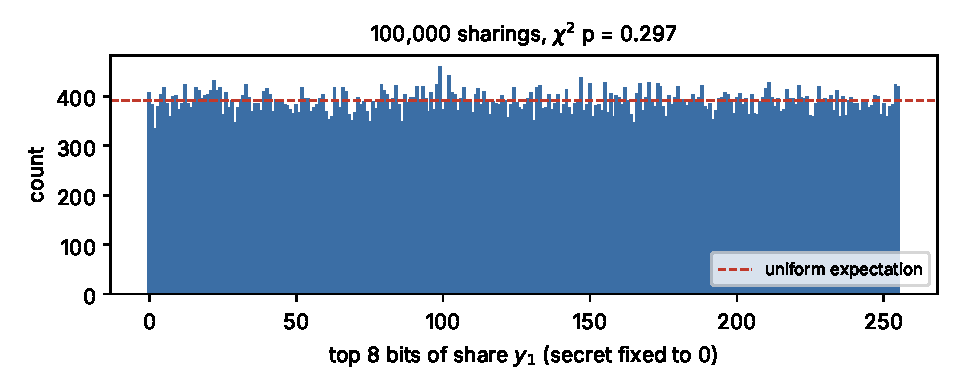
\includegraphics[width=0.78\textwidth]{figures/uniformity.pdf}
\caption{Distribution of the top byte of share $y_1$ over all sharings of a fixed secret (E2).}
\label{fig:uniformity}
\end{figure}

\paragraph{E3 Collusion with an SMT solver.} Given two of three needed shares, Z3 enumerated every
secret consistent with the view. Toy SAKSI ($p=31$, $t=3$): \EthreeSaksiCand{} of
\EthreeSaksiSpace{} candidates remain (\EthreeSaksiBits{} bits leaked). Mignotte control (moduli
$11,13,17,19,23$, threshold 3): \EthreeMigCand{} of \EthreeMigSpace{} candidates remain,
\EthreeMigBits{} bits leaked, which is why CRT-based sharing was not used.

\paragraph{E4 Forgery rate.} For nine toy primes from $5$ to $257$, \EfourTrials{} forgery attempts
each; the measured success rate tracks $1/p$ (largest absolute deviation \EfourMaxDev;
\cref{fig:forgery}), confirming \cref{thm:forge} is tight.

\begin{figure}[ht]
\centering
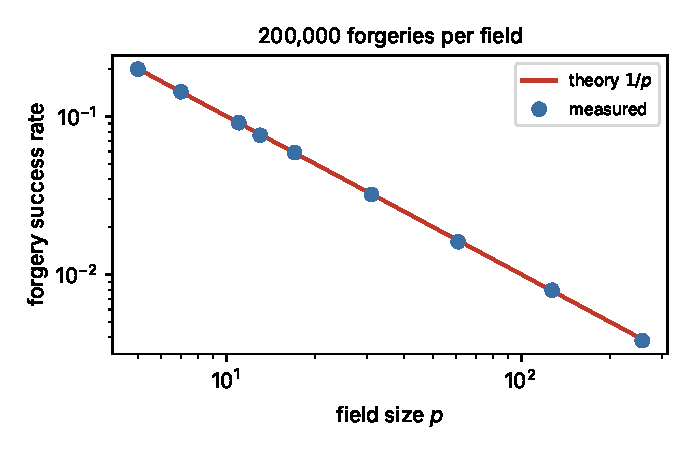
\includegraphics[width=0.55\textwidth]{figures/forgery.pdf}
\caption{Measured witness-forgery success vs.\ the bound $1/p$ (E4).}
\label{fig:forgery}
\end{figure}

\paragraph{E5 Active attacks at full size.} $p=2^{127}-1$, $n=5$, $t=3$, 32-byte key.
\Cref{tab:e5} compares plain Shamir (interpolate the first $t$ shares) with SAKSI.

\begin{table}[ht]
\centering\small
\begin{tabular}{@{}>{\raggedright\arraybackslash}p{5.0cm}rccc@{}}
\toprule
Attack & Trials & Control fooled & SAKSI wrong key & SAKSI names cheater \\
\midrule
bit flip in one share & 1000 & 81.9\% & 0.0\% & 100.0\% \\
random share replacement & 1000 & 100.0\% & 0.0\% & 100.0\% \\
Tompa--Woll: last submitter shifts share & 1000 & 100.0\% & 0.0\% & 100.0\% \\
cross-session substitution & 1000 & 100.0\% & 0.0\% & 100.0\% \\
two colluding cheaters, lying keys & 500 & 100.0\% & 0.0\% & 100.0\% \\
replay share from previous epoch & 500 & 100.0\% & 0.0\% & 100.0\% \\
inconsistent dealer (tags valid) & 500 & 100.0\% & 0.0\% & 100.0\% \\
\bottomrule
\end{tabular}

\caption{E5: rate at which each attack makes the system output a wrong key, and the rate at which
SAKSI names the cheater. ``Control fooled'' counts runs in which plain Shamir returned a wrong key.}
\label{tab:e5}
\end{table}

Every attack in \cref{tab:e5} was detected and attributed in all runs. Plain Shamir returned a
wrong key in all runs except for bit flips (\EfiveBitflip): with a 32-byte key the last limb holds
only 2 bytes, and when a flipped bit in that limb produces an error that stays inside its 13 bytes
of zero padding, the unvalidated control truncates the error away. SAKSI rejects those shares as
well, through the witness tags (and, as an extra, the padding check).

Two further rows probe the model's limits. \emph{Rushing control:} if keys are revealed before
shares (violating the protocol), the cheater recomputes valid tags and its forged share passes the
witness layer in \RushOneRound{} of \RushTrials{} runs, against \RushTwoRound{} with the SAKSI
order (\cref{prop:order}); in those one-round runs the independent syndrome layer still localised
the forged share and the correct key was output in \RushSyndrome{}. \emph{Bound tightness:} three
colluding custodians out of five ($c=3>T=2$) forge a consistent, well-formed alternative key,
vouch for each other and reject the honest shares. SAKSI then returned the coalition's wrong key in
\BoundWrong{} of \BoundTrials{} runs. This is the expected boundary, not a new weakness: robust
reconstruction is impossible against a dishonest majority, and with $c\ge t$ the coalition holds
the key anyway. The condition $c\le\lfloor(n-1)/2\rfloor$ in \cref{thm:robust} is tight.

\paragraph{E6 The same attacks on the Rust core.} \EsixTrials{} runs through the compiled
\texttt{saksi} binary (bit flip, Tompa--Woll shift, two cheaters): correct key \EsixCorrect{},
wrong key \EsixWrong{}, cheater named \EsixNamed{}.

\paragraph{E7 Fuzzing.} \EsevenN{} randomly mutated bundles (bad indices, non-canonical or
malformed field elements, truncated shares, duplicates, missing tags) fed to the Rust binary:
\EsevenCrash{} crashes and \EsevenWrong{} wrong keys returned.

\paragraph{E8 Timing of the Python reference (control).} The Python reference multiplies with
variable-time big integers. A dudect test (fixed $0$ vs.\ random, \EeightN{} samples) gives
$|t|=\EeightT$, i.e.\ it leaks. This is why the Python code is only the specification and test
oracle, and the deployable core is Rust (\cref{sec:sidechannel}).

\section{Side-channel engineering}\label{sec:sidechannel}

The track brief asks for an algorithm that resists side-channel attacks. The Rust core follows
four rules for every operation on secret data (source file \texttt{core/src/field.rs}).
\begin{enumerate}
  \item \textbf{Branch-free reduction.} Elements are canonical \texttt{u128} values. After an
  addition, the map $x\mapsto (x\bmod 2^{127})+\lfloor x/2^{127}\rfloor$ brings $x$ below $p+2$ (since
  $2^{127}\equiv1$), and the final conditional subtraction uses the borrow flag turned into an
  all-ones mask, never a branch.
  \item \textbf{Fixed-shape multiplication.} The $127\times127$-bit product is computed from four
  $64\times64\to128$-bit products; with $2^{128}\equiv2$ the $254$-bit result $h\cdot2^{128}+\ell$
  becomes $2h+(\ell\bmod2^{127})+\lfloor \ell/2^{127}\rfloor<2^{128}$, then is frozen as above.
  Measured cost: \BenchMul{}~ns.
  \item \textbf{Fixed ladder inversion.} $a^{-1}=a^{p-2}$ by a 127-step square-and-multiply ladder that
  \emph{always} multiplies and chooses the result with a masked select; the exponent is public, so
  the instruction trace is identical for every input (\BenchInv{}~$\mu$s).
  \item \textbf{Constant-time comparison and hygiene.} Tags are compared with an OR-reduction of
  $x\oplus y$ (\texttt{ct\_eq}); \texttt{core::hint::black\_box} prevents the compiler from turning
  masks back into branches; shares, keys, coefficients and reconstructed limbs are
  \texttt{zeroize}d on drop.
\end{enumerate}

\paragraph{Methodology.} We follow dudect~\cite{dudect17}: for each operation two input classes
(fixed vs.\ random) are generated \emph{before} measurement, interleaved in random order, timed
with serialised \texttt{rdtsc}, the slowest 5\% of each class discarded, and compared with Welch's
$t$-test; $|t|>4.5$ indicates a leak. Our first run generated the random inputs \emph{inside} the
timed region, so it measured the operating-system RNG and flagged every operation; we discarded it
and redid the study correctly. Two deliberately leaky functions serve as positive controls: an
extended-Euclid inverse and an early-exit byte comparison.

\begin{figure}[ht]
\centering
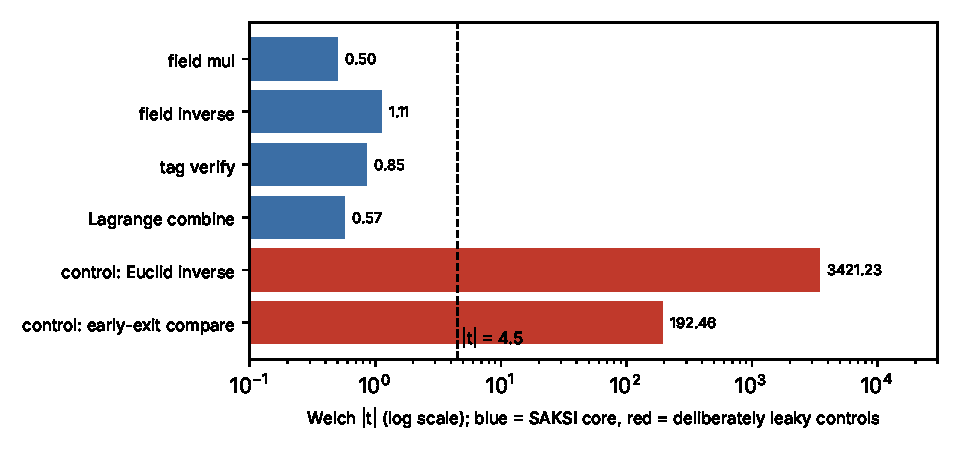
\includegraphics[width=0.85\textwidth]{figures/timing.pdf}
\caption{Welch $|t|$ per operation. SAKSI operations stay far below the 4.5 threshold; both leaky
controls are detected.}
\label{fig:timing}
\end{figure}

\begin{table}[ht]
\centering\footnotesize
\begin{tabular}{@{}lrrrl@{}}
\toprule
Operation (class A vs class B) & Samples & Mean A & Mean B & $|t|$ \\
\midrule
Fe::mul (fixed 0 vs random) & 1{,}000,000 & 88.6 & 88.6 & 0.50 \\
Fe::inv (fixed 1 vs random) & 250{,}000 & 4899.9 & 4899.9 & 1.11 \\
tag verify (valid vs forged tag) & 1{,}000,000 & 146.5 & 146.5 & 0.85 \\
Lagrange combine 3 shares (zero key vs random key) & 1{,}000,000 & 130.7 & 130.7 & 0.57 \\
\emph{control:} leaky Euclid inverse (fixed 1 vs random) & 250{,}000 & 135.1 & 2667.6 & 3421.23 \\
\emph{control:} leaky early-exit compare (equal vs random) & 1{,}000,000 & 90.1 & 85.9 & 192.46 \\
\bottomrule
\end{tabular}

\caption{dudect results for the Rust core (cycles). Class A is the fixed input, class B random.}
\label{tab:timing}
\end{table}

\paragraph{Limits.} Measurements were taken on a shared cloud virtual machine; they show the
absence of a \emph{detectable} leak at this sample size, not a proof. Constant-time behaviour
depends on the compiler, and the WebAssembly build in the browser demo runs under a JIT that gives
no constant-time guarantee. Gao decoding and polynomial division branch on degrees; they run only
when the syndrome is non-zero, and what they reveal (which shares are bad) is reported publicly
anyway. Power and electromagnetic channels are out of scope.

\section{Implementation and benchmarks}\label{sec:impl}

\begin{itemize}
  \item \textbf{Rust core} (\texttt{core/}): field, polynomials and Gao decoder, scheme, JSON wire
  format with input validation, CLI, and a WebAssembly build (\texttt{wasm-bindgen}). Tests: 4 unit
  and property-based tests of the field (256 random cases per property) and 10 integration tests of the
  scheme.
  \item \textbf{Python reference} (\texttt{ref/}): a direct transcription of
  \cref{fig:deal,fig:rec}; 18 tests. A cross-implementation check deals in one language and
  reconstructs in the other (30 rounds, identical results).
  \item \textbf{Performance} (release build, same VM): deal a 32-byte key 3-of-5 in
  \BenchDeal{}~$\mu$s; validated reconstruction from 5 shares in \BenchRec{}~$\mu$s; keyless
  decoding with one error in \BenchKeyless{}~$\mu$s.
\end{itemize}

\section{Applied environment: the Kunci Agent}\label{sec:applied}

To show the algorithm in use, the WebAssembly build of the core runs in a browser application
(\url{\demourl}). An API credential is dealt 3-of-5 to five custodians (the browser, a passkey- or
password-derived store, the server, and two simulated colleagues). A language-model agent (Gemini
through function calling, with Groq as a fallback provider) plans the user's task; when a step
needs the credential it calls a tool that runs the two-round SAKSI reconstruction, shows which
custodians were accepted, rejected or located, uses the key for a single outbound request and
zeroises it. The model only ever receives the tool's result; no share, tag, key or credential is
sent to the model provider. A ``tamper'' switch on each custodian lets a viewer reproduce the
attacks of \cref{sec:experiments} live. Source code: \url{\repourl}.

\section{Limitations}\label{sec:limits}
\begin{itemize}
  \item \textbf{Trusted dealer per epoch.} A dishonest dealer is caught if it hands out inconsistent
  shares, but a dealer that leaks the key is not prevented; dealer-free generation (each custodian
  dealing a sharing of a random contribution) is future work.
  \item \textbf{Key material grows as $\Theta(n^2L)$}, 432 bytes per custodian for $n=5$, $L=3$; fine
  for key custody, not for bulk data.
  \item \textbf{Honest majority.} Robustness needs $c\le\lfloor(n-1)/2\rfloor$; E5 shows what happens
  beyond it.
  \item \textbf{Ordered, authenticated channel to the combiner.} Proposition~\ref{prop:order} shows the
  order is essential; the combiner must enforce it. Duplicate submissions under one index are
  resolved by witness votes, but authenticated channels remain the clean assumption.
  \item \textbf{The key exists in memory at use.} Reconstruction necessarily materialises the key; we
  minimise the window and zeroise, but malware on the combining host can read it.
  \item \textbf{Refresh is centralised.} Our refresh uses one refresher; full mobile-adversary security
  needs a distributed refresh~\cite{herzberg95}.
  \item \textbf{Python is variable time} (E8) and is not meant for deployment.
  \item \textbf{The secret's length} $\lambda$ is public in the header.
\end{itemize}

\section{Compliance with the hackathon brief}\label{sec:brief}
\begin{itemize}
  \item \emph{Encrypts the master key without pre-existing algorithms:} the key is protected only by the
  SAKSI sharing itself (perfect secrecy); no block cipher, stream cipher, hash or library
  cryptography is used in the trust path. The only external dependency is the operating system's
  random number generator.
  \item \emph{Number theory:} arithmetic in the Mersenne field, $2^{127}\equiv1$ reduction, Fermat
  inversion, field-size forgery bounds.
  \emph{Linear algebra:} Vandermonde encoding, Lagrange coefficients, inner-product tags, the
  parity-check (syndrome) matrix and its rank argument, Reed--Solomon decoding.
  \item \emph{Low-level language:} the core is Rust with constant-time arithmetic.
  \item \emph{Applied environment:} the Kunci Agent (\cref{sec:applied}).
  \item \emph{Survives cryptanalysis / minimises attack surface:} \cref{sec:security,sec:surface,sec:experiments,sec:sidechannel}.
\end{itemize}

\begin{thebibliography}{99}\small
\bibitem{asmuthbloom83} C.~Asmuth and J.~Bloom. A modular approach to key safeguarding.
\emph{IEEE Transactions on Information Theory}, 29(2):208--210, 1983.
\bibitem{blakley79} G.~R.~Blakley. Safeguarding cryptographic keys. In \emph{Proc.\ National
Computer Conference (AFIPS)}, vol.~48, pages 313--317, 1979.
\bibitem{cfor12} A.~Cevallos, S.~Fehr, R.~Ostrovsky and Y.~Rabani. Unconditionally-secure robust
secret sharing with compact shares. In \emph{EUROCRYPT 2012}, LNCS 7237, pages 195--208, 2012.
\bibitem{feldman87} P.~Feldman. A practical scheme for non-interactive verifiable secret sharing.
In \emph{FOCS 1987}, pages 427--437, 1987.
\bibitem{gao02} S.~Gao. A new algorithm for decoding Reed--Solomon codes. In \emph{Communications,
Information and Network Security}, Springer, pages 55--68, 2003 (preprint 2002).
\bibitem{herzberg95} A.~Herzberg, S.~Jarecki, H.~Krawczyk and M.~Yung. Proactive secret sharing
or: how to cope with perpetual leakage. In \emph{CRYPTO '95}, LNCS 963, pages 339--352, 1995.
\bibitem{mignotte83} M.~Mignotte. How to share a secret. In \emph{Cryptography, Proc.\ Workshop
Burg Feuerstein 1982}, LNCS 149, pages 371--375, 1983.
\bibitem{pedersen91} T.~P.~Pedersen. Non-interactive and information-theoretic secure verifiable
secret sharing. In \emph{CRYPTO '91}, LNCS 576, pages 129--140, 1992.
\bibitem{rabinbenor89} T.~Rabin and M.~Ben-Or. Verifiable secret sharing and multiparty protocols
with honest majority. In \emph{STOC 1989}, pages 73--85, 1989.
\bibitem{dudect17} O.~Reparaz, J.~Balasch and I.~Verbauwhede. Dude, is my code constant time? In
\emph{DATE 2017}, pages 1697--1702, 2017.
\bibitem{rustsec} RustSec Advisory Database. RUSTSEC-2024-0398: Bias of polynomial coefficients in
secret sharing (crate \texttt{sharks}). 2024.
\bibitem{shamir79} A.~Shamir. How to share a secret. \emph{Communications of the ACM},
22(11):612--613, 1979.
\bibitem{tompawoll88} M.~Tompa and H.~Woll. How to share a secret with cheaters. \emph{Journal of
Cryptology}, 1(2):133--138, 1988.
\end{thebibliography}

\end{document}
